\chapter{Estrategia general del Análisis} \label{chap:ch4}

\newthought{Al estudiar fenómenos de nueva física}, es necesario definir una región en el espacio de fases de observables donde el modelo de señal BSM predice un exceso de eventos sobre el nivel de fondo. Esta región se llama Región de Señal (SR, \textit{Signal Region}), delimitada en este caso por el corte preliminar de selección en el puntaje del BDT sobre cada objeto DiTau, $BDT > 0.22$.

\begin{marginfigure}[55pt]
    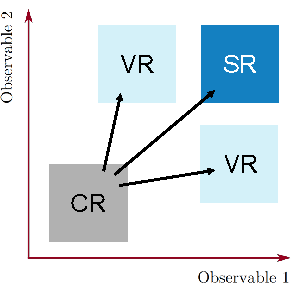
\includegraphics[width=0.99\linewidth]{Assets/Images/regions.pdf}
    \caption{Esquema genérico del diseño de las regiones de señal (SR), control (CR) y validación (VR) en términos de dos observables arbitrarios.}
    \label{fig:ch4:regions_generic}
\end{marginfigure}

El análisis de búsqueda consiste en estimar las contribuciones de los procesos del SM que contaminan la SR. Para esto existen tres técnicas principales: utilizar directamente simulaciones Monte Carlo (MC), en general solo para procesos despreciables en la SR; utilizar simulaciones MC corregidas con datos en regiones de control --como se explica más adelante-- para los procesos de fondo dominantes; o utilizar métodos \textit{data-driven}, basados en los propios datos observados. Estos últimos están especialmente destinados a la estimación de fondos correspondientes a objetos físicos identificados erróneamente como otras partículas.

Estos fondos simulados dominantes requieren una normalización con respecto a los datos, corrigiendo desviaciones en el modelado teórico por medio de factores de transferencia $\mu_{\text{fondo}}$. Para esto se definen Regiones de Control (CRs, \textit{Control Regions}), ortogonales a las SRs, buscando maximizar en cada caso los eventos de un fondo en particular. Luego de haber estudiado los fondos contribuyentes se realiza un ajuste multivariable de distintas distribuciones de observables en todas las CRs y el valor final de los factores de transferencia de cada proceso es establecido.

Las estimaciones de los distintos fondos y los métodos utilizados en su cálculo son verificadas en Regiones de Validación (VRs, \textit{Validation Regions}). Estas regiones se encuentran próximas a las CRs y SRs en el espacio de fase, aunque sin solaparse, como podemos observar en el esquema exhibido en la \cref{fig:ch4:regions_generic}. El diseño de las VRs comprende un compromiso entre minimizar la contaminación de la señal, y al mismo tiempo ser efectivas en la validación de la extrapolación entre CRs y SRs.

En este capítulo describiremos la estrategia general del análisis, enunciando un primer conjunto de cortes de selección (preselección). Introduciremos los fondos contaminantes al estado final de la resonancia de baja masa de la búsqueda, listando las muestras de MC necesarias para su estimación y las Regiones de Control necesarias para la normalización del fondo dominante. Finalmente, daremos una primera definición de la región de señal.


\section{Procesamiento de las muestras simuladas y datos} \label{sec:ch4:processing}

El presente análisis de búsqueda comprende el uso de datos experimentales colectados por el detector ATLAS durante el Run 2 del LHC, con una energía de centro de masa de $\sqrt{s} = \SI{13}{\TeV}$. Luego de imponer requerimientos de calidad en los eventos colectados, se dispone de una luminosidad integrada total de \SI{139}{\femto\barn^{-1}}. Sin embargo, al tratarse del primer estudio sobre los fondos contaminantes en el análisis, para agilizar las iteraciones en su desarrollo, en este trabajo solo se utilizaron simulaciones de Monte Carlo y datos experimentales del año 2017 (\SI{44.3}{\femto\barn^{-1}}).

Las simulaciones de Monte Carlo de los procesos de fondo y señal fueron realizadas utilizando una simulación del detector ATLAS en el software Geant4~\cite{TheATLASCollaboration2010}. Las muestras fueron desarrolladas por el \textit{Physics Modelling Group} de ATLAS como parte de la campaña de simulación denominada internamente \texttt{mc16d}, modelando las condiciones de adquisición de datos del año 2017. Los procesos de señal $t\bar{t}(X\to\tau\tau)$ fueron obtenidos utilizando el modelo 2HDM, configurado como se indica en el \cref{ap:ap1}, generando $10^5$ eventos para masas del pseudoescalar $h_3$ de \num{20}, \num{40} y \SI{60}{\GeV}; se consideraron decaimientos semileptónicos y totalmente leptónicos del par $t\bar{t}$. Las secciones eficaces de las muestras y la configuración de los generadores se encuentran en la \cref{tbl:ch4:MC_samples:signal}.

Las incertezas estadísticas de los procesos del SM y datos fueron calculadas considerando un intervalo de confianza de 68\% en una distribución de Poisson. No se han estudiado todavía las incertezas sistemáticas en este análisis.

\begin{sidewaystable}
    \vspace{18.5em}
    \subfloat[][Muestras de fondo \label{tbl:ch4:MC_samples:bkg}]{\noindent\makebox[\textwidth]{\small\centering\begin{tabular}{L{35mm} C{28mm}C{28mm}C{28mm}C{14mm}C{23mm}C{25mm}C{24mm}}
\toprule
%\multicolumn{1}{c}{Process} & DSIDs         & Cross Section (\si{\pico\barn})   & Event generator & ME order & Parton shower & PDF            & Tune           \\
\multicolumn{1}{c}{Proceso} & DSIDs         & Sección eficaz (\si{\pico\barn})  & Generador       & Órden ME & Parton shower & PDF            & Tune           \\
\midrule
$t\bar{t}$                  & 410470        & 729.77                            & Powheg          & NLO      & Pythia 8      & NNPDF 3.0 NLO  & A14            \\
Single Top $t$-channel      & 410560        & 0.24041                           & MadGraph5\_aMC  & NLO      & Pythia 8      & NNPDF 3.0 NLO  & A14            \\
                            & 410658-410659 & 59.169                            & Pweheg          & NLO      & Pythia 8      & NNPDF 3.0 NLO  & A14            \\
Single Top $s$-channel      & 410644-410645 & 3.2944                            & Pweheg          & NLO      & Pythia 8      & NNPDF 3.0 NLO  & A14            \\
Single Top $Wt$-channel     & 410646-410647 & 75.840                            & Pweheg          & NLO      & Pythia 8      & NNPDF 3.0 NLO  & A14            \\
$t\bar{t}t$                 & 304014        & 0.0016396                         & MadGraph5\_aMC  & LO       & Pythia 8      & NNPDF 2.3 LO   & A14            \\
$t\bar{t}t\bar{t}$          & 410080        & 0.0091626                         & MadGraph5\_aMC  & LO       & Pythia 8      & NNPDF 2.3 LO   & A14            \\
$t\bar{t}H$                 & 345874        & 0.54945                           & Powheg          & NLO      & Pythia 8      & NNPDF 3.0 NLO  & A14            \\
$t\bar{t}W$                 & 410155        & 0.54822                           & MadGraph5\_aMC  & NLO      & Pythia 8      & MEN 3.0 NLO    & A14            \\
$t\bar{t}Z$                 & 410157        & 0.52821                           & MadGraph5\_aMC  & NLO      & Pythia 8      & MEN 3.0 NLO    & A14            \\
$t\bar{t}ee$                & 410218        & 0.036864                          & MadGraph5\_aMC  & LO       & Pythia 8      & NNPDF 2.3 LO   & A14            \\
$t\bar{t}\mu\mu$            & 410219        & 0.036868                          & MadGraph5\_aMC  & LO       & Pythia 8      & NNPDF 2.3 LO   & A14            \\
$t\bar{t}\tau\tau$          & 410220        & 0.036555                          & MadGraph5\_aMC  & LO       & Pythia 8      & NNPDF 2.3 LO   & A14            \\
$W(\to \mu\nu) + Jets$      & 364156-364169 & 60581                             & Sherpa 2.1.1    & NNLO     & Sherpa        & NNPDF 3.0 NNLO & Sherpa default \\
$W(\to e\nu) + Jets$        & 364170-364183 & 61533                             & Sherpa 2.1.1    & NNLO     & Sherpa        & NNPDF 3.0 NNLO & Sherpa default \\
$W(\to \tau\nu) + Jets$     & 364184-364197 & 61545                             & Sherpa 2.1.1    & NNLO     & Sherpa        & NNPDF 3.0 NNLO & Sherpa default \\
$Z(\to \mu\mu) + Jets$      & 364100-364113 & 6420.5                            & Sherpa 2.1.1    & NNLO     & Sherpa        & NNPDF 3.0 NNLO & Sherpa default \\
$Z(\to ee) + Jets$          & 364114-364127 & 6426.9                            & Sherpa 2.1.1    & NNLO     & Sherpa        & NNPDF 3.0 NNLO & Sherpa default \\
$Z(\to \tau\tau) + Jets$    & 364128-364141 & 6427.8                            & Sherpa 2.1.1    & NNLO     & Sherpa        & NNPDF 3.0 NNLO & Sherpa default \\
Diboson Fully-Leptonic      & 361600-361602 & 17.896                            & Pweheg          & NLO      & Pythia 8      & NNPDF 3.0 NLO  & A14            \\
                            & 361604-361605 & 1.4710                            & Pweheg          & NLO      & Pythia 8      & NNPDF 3.0 NLO  & A14            \\
Diboson Semi-Leptonic       & 361606-361611 & 69.554                            & Pweheg          & NLO      & Pythia 8      & NNPDF 3.0 NLO  & A14            \\
\bottomrule
\end{tabular}}}\\

    \vspace{1em}

    \subfloat[][Muestras de señal \label{tbl:ch4:MC_samples:signal}]{\noindent\makebox[\textwidth]{\small\centering\begin{tabular}{L{35mm} C{28mm}C{28mm}C{28mm}C{14mm}C{23mm}C{25mm}C{24mm}}
\toprule
\multicolumn{1}{c}{Proceso}                  & DSIDs         & Sección eficaz (\si{\pico\barn})  & Generador       & Órden ME & Parton shower & PDF            & Tune           \\
\midrule
$t\bar{t}(X\to\tau\tau)$ \ @ \ \SI{20}{\GeV} & 345919        & 0.00024634                        & MadGraph5\_aMC  & NLO      & Pythia 8      & NNPDF 2.3 LO   & A14            \\
$t\bar{t}(X\to\tau\tau)$ \ @ \ \SI{40}{\GeV} & 345920        & 0.00042478                        & MadGraph5\_aMC  & NLO      & Pythia 8      & NNPDF 2.3 LO   & A14            \\
$t\bar{t}(X\to\tau\tau)$ \ @ \ \SI{60}{\GeV} & 345928        & 0.00054083                        & MadGraph5\_aMC  & NLO      & Pythia 8      & NNPDF 2.3 LO   & A14            \\
\bottomrule
\end{tabular}}}
    
    \vspace{1em}

    \caption{Muestras de MC utilizadas en la estimación de los fondos \subref{tbl:ch4:MC_samples:bkg}, y simulaciones de la señal \subref{tbl:ch4:MC_samples:signal}, de la campaña de simulaciones \texttt{mc16d} con las condiciones de funcionamiento del LHC en el año 2017. \textit{DSID} refiere al código identificador interno de las muestras. \textit{Tune} refiere a la configuración de los parámetros de la simulación de las lluvias partónicas. Las PDF enunciadas en la tabla corresponden a los elementos de matriz (ME). La PDF usada en las lluvias partónicas es ``NNPDF 2.3 LO'' en todas las muestras que emplean el \text{tune} A14, y la PDF por defecto en todas las muestras producidas por Sherpa.}
    \label{tbl:ch4:MC_samples}
\end{sidewaystable}

La producción de NTuplas fue realizada con una versión extensamente modificada del framework \texttt{XAMPP}\sidenote{Este programa, desarrollado inicialmente por el Instituto Max Plank de Física de Munich, se utiliza como base de los frameworks de muchos análisis de búsqueda de partículas escalares.} ejecutando la identificación de los objetos DiTau utilizando el BDT, la calibración de los objetos físicos y la preselección de los eventos utilizados en el análisis.

La selección final de eventos, su análisis y la producción de histogramas se realizó con un software basado en ROOT e implementado en C++ y Python, desarrollado como parte del presente trabajo de tesis.

Las simulaciones son producidas independientemente de la luminosidad y la sección eficaz del proceso del SM subyacente, usualmente requiriendo la generación de número fijo de eventos por cada proceso y canal. Por lo tanto, las muestras de MC deben ser escaladas a la luminosidad del período al que pertenecen los datos experimentales y la sección eficaz teórica, calculada por separado. Todos los eventos simulados reciben un factor de escala
\begin{align}
    w &= \frac{\int L \dd{t}}{\text{TotalSumW}} \times \text{xSection} \times \text{kFactor} \times \text{FilterEfficiency} \times \text{GenWeight} \nonumber \\
        &\quad\quad \times \text{muWeight} \times \text{LeptonWeight} \times \text{JetWeight}. \label{eq:ch4:weight}
\end{align}
En particular, el factor de normalización \textit{TotalSumW} es la suma de los pesos pre-existentes y $\int L \dd{t}$ es la luminosidad integrada total de los datos a los que serán comparados. Los factores \textit{xSection}, \textit{kFactor} y \textit{FilterEfficiency}, se corresponden a la sección eficaz teórica de cada proceso, correcciones provenientes de la omisión de términos de orden superior en los cálculos incluidos en las simulaciones y las eficiencias de los filtros aplicados a los eventos generados. Los siguientes términos, \textit{GenWeight} y \textit{muWeight}, representan correcciones debidas a la generación y al pileup de cada evento.

Los últimos términos, \textit{JetWeight}, \textit{EleWeight} y \textit{MuoWeight}, corrigen diferencias en la eficiencia de procesamiento de cada objeto, entre simulaciones y datos\sidenote[][-6em]{Para cada objeto incluido en el análisis
\[ \text{ObjWeight} = \prod_{i} \frac{N_i(\text{Datos})}{N_i(\text{MC})}, \]
donde la productoria es sobre todos los procesos inplicados en el procesamiento de cada objeto: reconstrucción, identificación, aislamiento, trigger y otros.
}. Solo se incluyen los pesos de los objetos presentes en cada evento: en aquellos donde no se han reconstruido alguno de estos objetos, el factor correspondiente se asigna a 1. Los pesos de los objetos DiTau están siendo determinados por otro grupo de trabajo, estudiando eventos \textit{Truth Matched} en el proceso $Z(\to\tau\tau) + \gamma/Jets$, con un fotón \textit{prompt} producido en asociación al $Z$. Se espera una dependencia de este factor con el score del BDT, que deberá ser considerada.





\noFBSection{Preselección de eventos} \label{sec:ch4:presel_cuts}

Aplicamos una preselección de objetos candidatos a las partículas del proceso en todos los eventos, basada en la topología y las propiedades del estado final de los eventos $tt(X\to\tau_h\tau_h)$ con $X$ boosteado, exhibido en la \cref{fig:ch4:ttX_diagram}. En esta búsqueda estudiamos eventos donde el par $t\bar{t}$ asociado a la producción del $X$ decae semileptónicamente. En este canal de decaimiento, solo uno de los quarks top decae leptonicamente a $e/\mu + \nu_e/\nu_\mu$ a través de la producción de un $W^\pm$ y un quark $b$, mientras que el otro resulta en 3 quarks, uno de los cuales debe ser también un quark $b$ y los otros dos provienen del $W^\pm$ decayendo hadrónicamente. Por lo tanto, se espera un único leptón en todos los eventos.

\begin{marginfigure}
    \resizebox{\linewidth}{!}{\ttXdiagram}
    \caption{Diagrama de Feynman de un evento $t\bar{t}(X \to \tau_h \tau_h)$, con $X$ boosteado, con decaimiento semileptónico del par $t\bar{t}$.}
    \label{fig:ch4:ttX_diagram}
\end{marginfigure}

El leptón de trigger deberá completar alguna de las siguientes cadenas de Trigger L1 y HLT sin factores de pre-escala (\textit{unprescaled}), separadas por $p_T$ mínimo y WP de reconstrucción y aislamiento de los objetos~\cite{TheATLASCollaboration2020a,Rettie2018}:
\begin{itemize}
    \item \textsc{Triggers de {\footnotesize 1} electrón:}
    \begin{itemize}
        \small
        \item \texttt{HLT\_e26\_lhtight\_nod0\_ivarloose}: con $p_T > \SI{26}{\GeV}$, identificación \textit{tight} y aislamiento \texttt{loose} de radio variable.
        \item \texttt{HLT\_e60\_lhmedium\_nod0}: con $p_T > \SI{60}{\GeV}$ e identificación \textit{medium} sin aislamiento
        \item \texttt{HLT\_e140\_lhloose\_nod0}: con $p_T > \SI{140}{\GeV}$ e identificación \textit{loose} sin aislamiento,
    \end{itemize}
    \item \textsc{Triggers de {\footnotesize 1} muón:}
    \begin{itemize}
        \small
        \item \texttt{HLT\_mu26\_ivarmedium}: con $p_T > \SI{26}{\GeV}$, identificación \textit{medium} y aislamiento \textit{medium} de radio variable,
        \item \texttt{HLT\_mu50}: con $p_T > \SI{50}{\GeV}$ e identificación \textit{medium} sin aislamiento,
        \item \texttt{HLT\_mu60\_0eta105\_msonly}: con $p_T > \SI{60}{\GeV}$, identificación \textit{medium} sin aislamiento, reconstruido utilizando solo trazas del MS en la región \textit{barrel}.
    \end{itemize}
\end{itemize}
En todos los triggers de electrones, \texttt{nod0} indica que no se requieren cortes en el parámetro de impacto transversal $\abs{d_0 \sin\theta}$. Se requiere una coincidencia entre los leptones utilizados en el trigger y los electrones y muones reconstruidos \textit{offline}, conocida como \textit{trigger matching}.

Las NTuplas cuentan con dos especificaciones de leptones progresivamente más restrictivas\sidenote{Todo leptón etiquetado como \textit{signal} también satisfará los requerimientos de \textit{baseline}.}, denominadas \textit{baseline} y \textit{signal}, con diferentes cortes cinemáticos, WP de identificación (ID) y aislamiento (Iso) de los objetos físicos. A partir de la cinemática de los eventos de señal, solo se consideran electrones y muones con $p_T > \SI{27}{\GeV}$. Los leptones \textit{signal} de $p_T > \SI{300}{\GeV}$ pueden especificar un requerimiento de aislamiento adicional (IsoHighPt); en el caso de los electrones se elije un WP más estricto, solo utilizando información del ECal. Un resumen completo de los cortes de selección se encuentran en la \cref{tbl:ch4:presel:leptons}.

Los jets y b-jets empleados en el análisis son jets anti-$k_t$ reconstruidos con el algoritmo Particle Flow y calibración de energía electromagnética, en todos los casos pasando el WP \textit{tight} del JVT. Los cortes cinemáticos y de calidad se encuentran en la \cref{tbl:ch4:presel:(b)jets}.

En los casos en que un objeto físico es reconstruido e identificado erróneamente como múltiples tipos de partículas simultáneamente, se aplica un procedimiento de eliminación de superposiciones (OR, \textit{Overlap Removal}). Esto es realizado por el framework de producción de NTuplas entre electrones, muones y jets, aunque deberá ser ejecutado manualmente en el caso de los objetos DiTau. En el caso de los jets, se rechazan todos aquellos objetos que intersecten al cono exterior del objeto DiTau, requiriendo $\Delta R(\text{DiTau}, \text{Jet}) > 1.0$, para evitar un doble-conteo. Una vez completado el OR, se aplica un corte sobre el número de jets y b-jets, eliminando eventos con menos de $2$ jets y sin b-jets.

Todos los eventos deberán contener al menos 1 objeto DiTau de $p_T > \SI{50}{\GeV}$ con al menos 2 subjets, cada uno con 1 o 3 trazas en su interior. Se aplica un requerimiento adicional sobre las cargas de los subjets LyS $\abs{q} == 1$, para discriminar objetos mal reconstruidos, como se indica en la \cref{tbl:ch4:presel:ditaus}.

\begin{table}[t]
    \small\centering
    \setlength{\tabcolsep}{1mm}
    \begin{tabular}{L{15mm} C{20mm}C{24mm}C{20mm}C{20mm}}
\toprule
                        & \multicolumn{2}{c}{Electrones}                    & \multicolumn{2}{c}{Muones}                     \\
                        & Baseline              & Signal                    & Baseline             & Signal                  \\
\midrule
$N$                     & \multicolumn{4}{c}{1 leptón etiquetado \textit{Signal}}                                            \\
$p_T$                   & \multicolumn{2}{c}{$\geq \SI{27}{\GeV}$}          & \multicolumn{2}{c}{$\geq \SI{27}{\GeV}$}       \\
$\abs{\eta}$            & \multicolumn{2}{c}{$\leq 2.47$}                   & \multicolumn{2}{c}{$\leq 2.5$}                 \\
ID                      & \texttt{VeryLooseLLH} & \texttt{MediumLLH}        & \texttt{Medium}      & \texttt{Medium}         \\
Iso                     & ---                   & \texttt{FCLoose}          & ---                  & \texttt{Loose\_VarRad}  \\
IsoHighPt               & ---                   & \texttt{FCHighCaloOnly}   & ---                  & \texttt{Loose\_VarRad}  \\
$\abs{z_0 \sin\theta}$  & ---                   & $< 0.5$                   & $< 0.5$              & $< 0.5$                 \\
$d_0$                   & ---                   & $< 5$                     & ---                  & $< 3$                   \\
\bottomrule
\end{tabular}

    \caption{Criterios de preselección de leptones en eventos $t\bar{t}(X\to\tau\tau)$, con decaimiento semi-leptónico del $t\bar{t}$.}
    \label{tbl:ch4:presel:leptons}
    \setfloatalignment{b}
\end{table}

\begin{table}[t]
    \small\centering
    \setlength{\tabcolsep}{1mm}
    \begin{tabular}{L{15mm} C{90mm}}
\toprule
                    & (B)Jets                                                                              \\
\midrule
$N$                 & $\geq 2$                                                                             \\
$p_T$               & $\geq \SI{20}{\GeV}$                                                                 \\
$\abs{\eta}$        & $\leq 2.5$                                                                           \\
Tipo                & \texttt{AKt4EMPFlow}                                                                 \\
JVT                 & \texttt{Tight JVT}, $JVT > 0.5$ si $p_T < \SI{60}{\GeV}$ \&\& $\abs{\eta} \leq 2.4$  \\
B-Tagging           & \texttt{MV2c10}, WP 85\% si $\abs{\eta} \leq 2.5$ \&\& $p_T \geq \SI{20}{\GeV}$      \\
$N_{\text{BJets}}$  & $\geq 1$                                                                             \\
\bottomrule
\end{tabular}

    \caption{Criterios de preselección de jets y b-jets en eventos $t\bar{t}(X\to\tau\tau)$, con decaimiento semi-leptónico del $t\bar{t}$. Los números de jets y b-jets (\textit{NJets} y \textit{NBJets}) son calculados luego de remover su solapamiento con los objetos DiTau requiriendo $\Delta R(\text{DiTau}, \text{Jet}) > 1.0$ (los jets deben encontrarse fuera del cono de radio $R = 1.0$ del DiTau).}
    \label{tbl:ch4:presel:(b)jets}
    \setfloatalignment{b}
\end{table}

\begin{table}[t]
    \small\centering
    \setlength{\tabcolsep}{1mm}
    \begin{tabular}{L{15mm} C{90mm}}
\toprule
             & DiTaus                                                           \\
\midrule
$N$          & $\geq 1$                                                         \\
$p_T$        & $\geq \SI{50}{\GeV}$                                             \\
$\abs{\eta}$ & $\leq 2.5$                                                       \\
Tracks       & $1 \ || \ 3$, en subjets \textit{leading} y \textit{subleading}  \\
Cargas       & $|q| == 1$, en subjets \textit{leading} y \textit{subleading}    \\
\bottomrule
\end{tabular}

    \caption{Criterios de preselección de DiTaus en eventos $t\bar{t}(X\to\tau\tau)$, con decaimiento semi-leptónico del $t\bar{t}$.}
    \label{tbl:ch4:presel:ditaus}
    \setfloatalignment{b}
\end{table}





\noFBSection{Procesos de fondo contaminantes} \label{sec:ch4:bkg_processes}

Para poder detectar la presencia de señal de nueva física en las mediciones experimentales, es necesaria una buena estimación de los procesos del Modelo Estándar conocidos con un estado final compatible al de la señal buscada (\cref{fig:ch4:ttX_diagram}). Estos procesos, que conforman el fondo de SM, deben contener objetos que puedan ser reconstruidos y mal-identificados como un objeto DiTau \textit{fake}. Además, los procesos de fondo deberán incluir al menos un leptón $e^\pm$ o $\mu^\pm$ en su estado final, para ser compatibles con el trigger.

Existen muchos procesos del SM que pueden contribuir a los fondos, pero los principales comprenden la producción de quarks top y bosones vectoriales. En el caso de eventos que incluyen quarks $t$, se espera iniciar el trigger con uno de los leptones producidos en el decaimiento de uno de los quarks (como en $t\bar{t}$), o adicionalmente del decaimiento de una de las partículas producidas en asociación con los quarks $t$ (como en el proceso $t\bar{t}W$, donde $W\to\ell\nu$). Los principales procesos que se contemplan en esta categoría son:
\begin{itemize}
    \item $t\bar{t}$. Se espera que esta sea la contribución de fondo dominante, debido a su similitud con el proceso de señal (\cref{fig:ch4:ttX_diagram,fig:ch4:ttbar_diagram}) y a su elevada sección eficaz sobre los otros procesos.
    \item Single Top ($s$-channel, $t$-channel y $Wt$-channel).
    \item $t\bar{t}t$ (3t) y $t\bar{t}t\bar{t}$ (4t).
    \item $t\bar{t}H$, $t\bar{t}W$, $t\bar{t}Z$ (solo en decaimiento a quarks).
    \item $t\bar{t}ee$, $t\bar{t}\mu\mu$ y $t\bar{t}\tau\tau$, por medio de la producción de un $Z$.
\end{itemize}

\begin{marginfigure}[-10em]
    \resizebox{0.99\linewidth}{!}{\begin{tikzpicture}[font=\Large]
    \begin{feynman}
        \vertex (g1) at (0,0) {$g$};
        \vertex[right=30mm of g1] (g1_t);
        \vertex[above right=15mm and 43mm of g1_t] (W1_end);
        \vertex[above right=5mm and 5mm of W1_end] (l) {$\ell$};
        \vertex[below right=5mm and 5mm of W1_end] (nu) {$\bar{\nu}_\ell$};
        \vertex (W1_start) at ($(g1_t)!0.77!(W1_end) + (0mm, -1mm)$);
        \vertex[below right=5mm and 5mm of W1_start] (b1) {$b$};
        %
        \vertex[below=20mm of g1] (g2) {$g$};
        \vertex[right=30mm of g2] (g2_t);
        \vertex[below right=15mm and 43mm of g2_t] (W2_end);
        \vertex[above right=5mm and 5mm of W2_end] (q1) {$q$};
        \vertex[below right=5mm and 5mm of W2_end] (q2) {$\bar{q}$};
        \vertex (W2_start) at ($(g2_t)!0.77!(W2_end) + (0mm, +1mm)$);
        \vertex[above right=5mm and 5mm of W2_start] (b2) {$\bar{b}$};
        %
        \diagram*{
        (g1) -- [gluon] (g1_t),
        (g2) -- [gluon] (g2_t),
        %
        (b2) -- [fermion] (W2_start) -- [fermion, edge label={$\bar{t}$}] (g2_t) -- [fermion] (g1_t) -- [fermion, edge label={$t$}] (W1_start) -- [fermion] (b1),
        %
        (W1_start) -- [boson, edge label={$W^+$}] (W1_end),
        (nu) -- [fermion] (W1_end) -- [fermion] (l),
        %
        (W2_start) -- [boson, edge label'={$W^-$}] (W2_end),
        (q2) -- [fermion] (W2_end) -- [fermion] (q1),
        };
    \end{feynman}
\end{tikzpicture}}
    \caption{Diagrama de Feynman de un evento $t\bar{t}$ semileptónico.}
    \label{fig:ch4:ttbar_diagram}
\end{marginfigure}

En el caso de procesos relacionados a la producción directa de bosones vectoriales, el trigger puede ser iniciado por un leptón ($e$ o $\mu$) proveniente del decaimiento de los bosones $W^\pm$ y $Z^0$. En los decaimientos $W\to\tau\nu$ y $Z\to\tau\tau$, el trigger será iniciado en el decaimiento leptónico de uno de los \ttau. Los procesos considerados son:
\begin{itemize}
    \item $Z(\to \ell\ell / \tau\tau) + Jets$\sidenote{Por convención en ATLAS se suele referir como ``leptones'' solamente a los electrones y muones, por lo que $\ell = e, \mu$.},
    \item $W(\to \ell\nu / \tau\nu) + Jets$,
    \item DiBoson ($WW$, $WZ$ y $ZZ$ en los decaimientos semi-leptónicos y totalmente leptónicos).
\end{itemize}

Las secciones eficaces de las muestras y la configuración de los generadores se encuentran en la \cref{tbl:ch4:MC_samples:bkg}.

Existen otras contribuciones a los fondos, provenientes de partículas identificadas incorrectamente como objetos DiTau y leptones utilizados para el trigger. El modo dominante proviene del fondo Multijet, compuesto por jets de QCD sin leptones ni fotones \textit{prompt}, donde reconstruimos un leptón \textit{fake} y un objeto DiTau \textit{fake} en un mismo evento. Su estimación se realiza preliminarmente con simulaciones de MC, aunque se deben corregir y validar utilizando métodos \textit{data-driven} en la etapa final de estimación de los fondos para el análisis. Estos fondos no están incluidos en los resultados preliminares exhibidos en este trabajo.





\noFBSection{Distribuciones de preselección} \label{sec:ch4:presel_results}

\begin{figure*}[t]
    \centering
    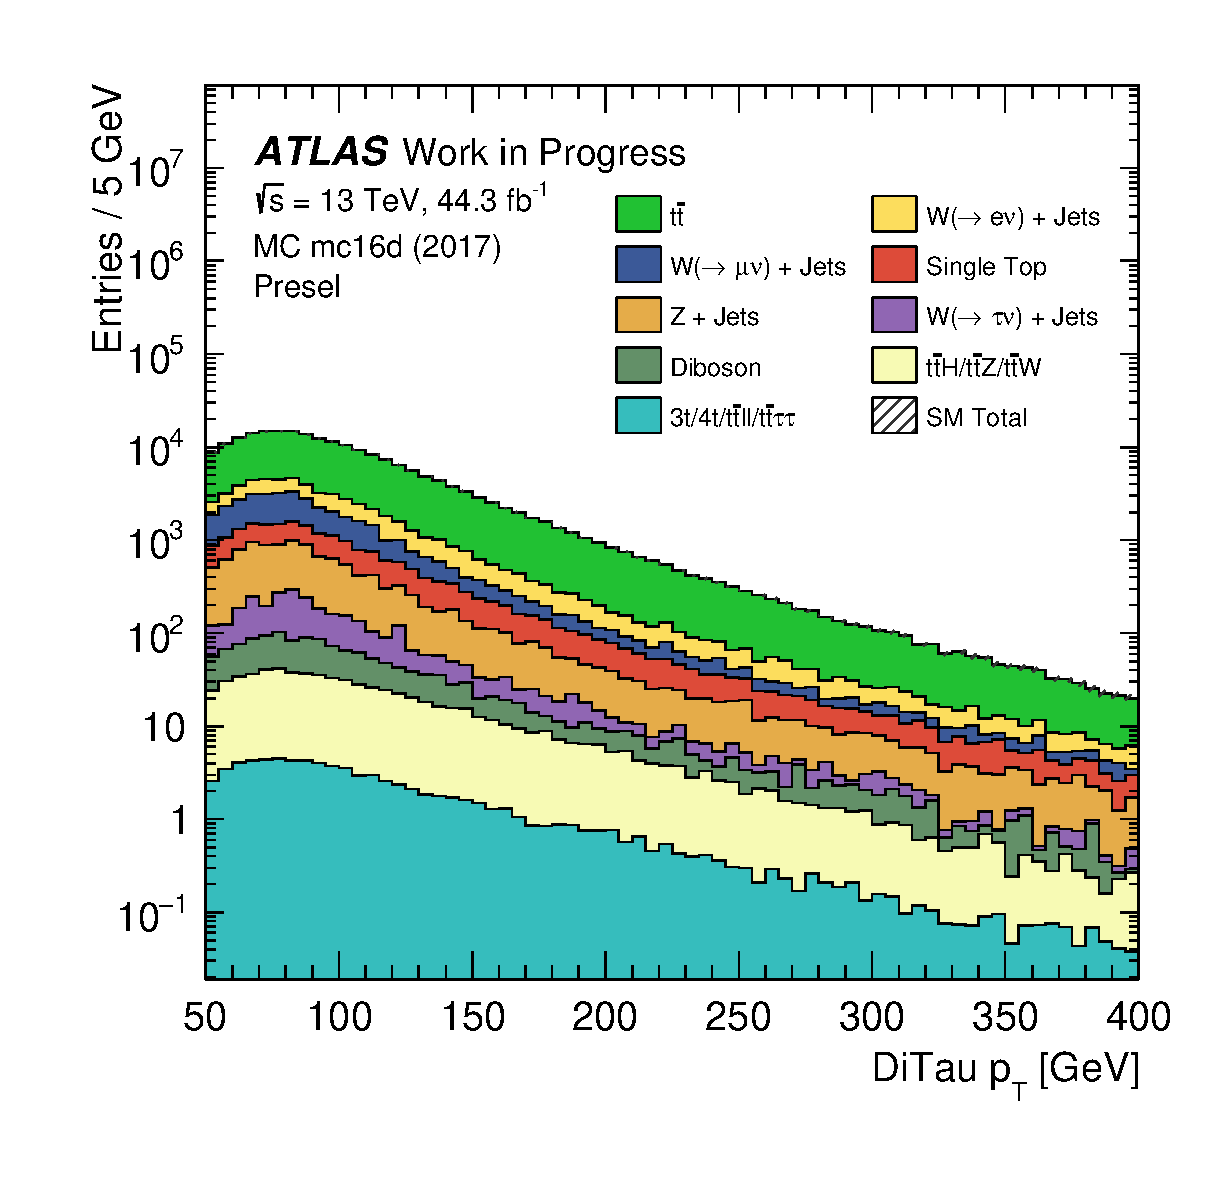
\includegraphics[width=0.49\fulllinewidth]{Assets/Plots/Presel/h_stack_mc16d_ditau_pt.eps}
    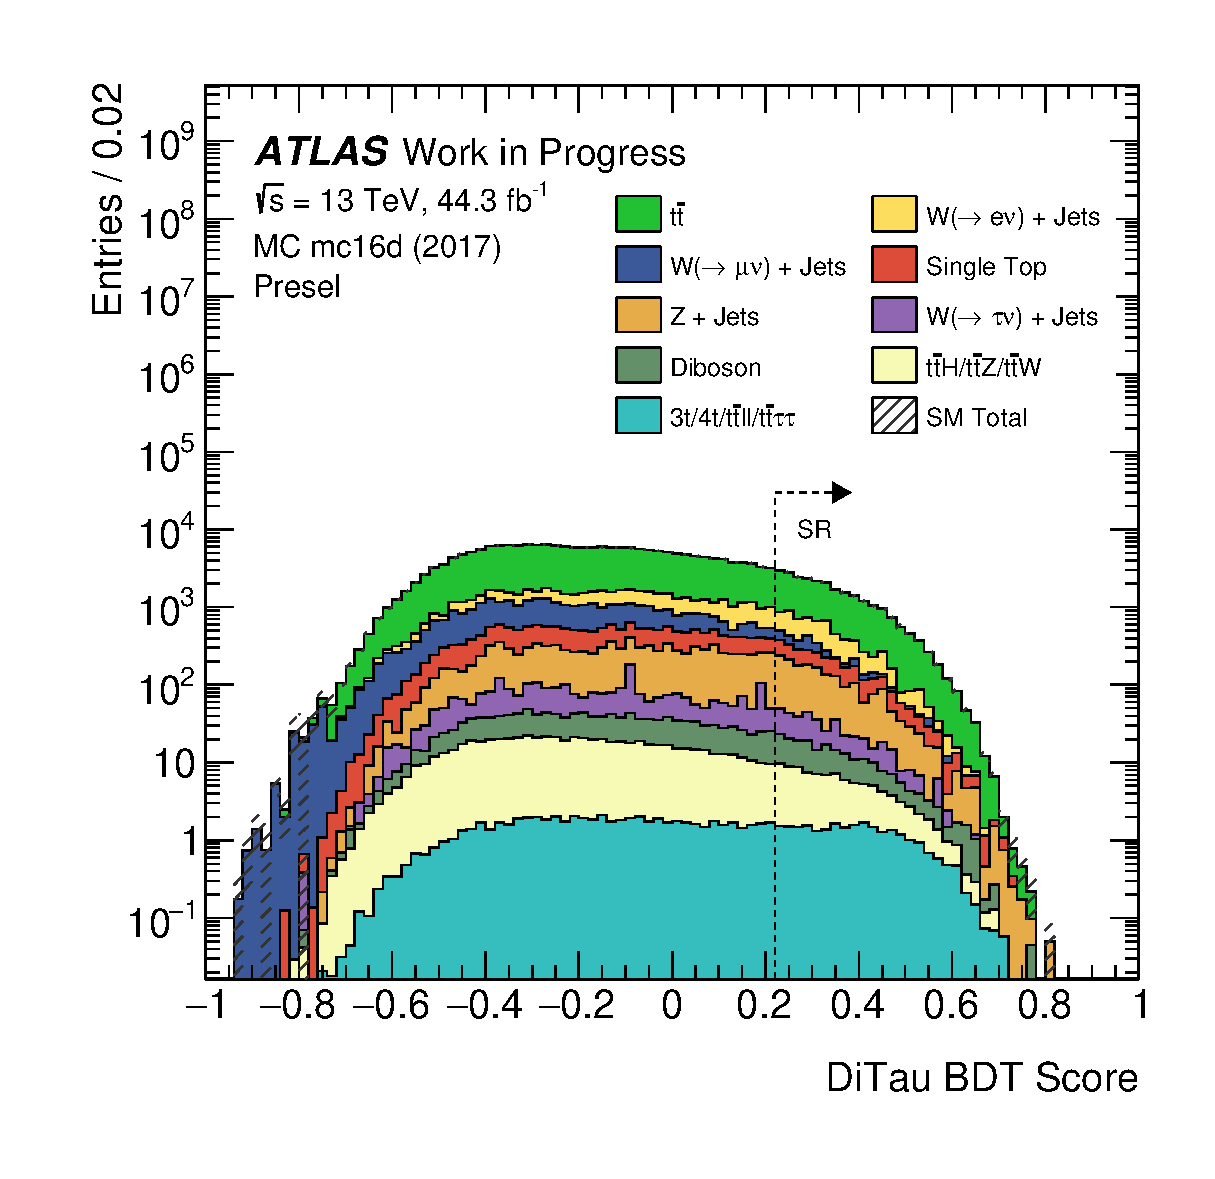
\includegraphics[width=0.49\fulllinewidth]{Assets/Plots/Presel/h_stack_mc16d_ditau_bdt.eps}

    \caption{Distribuciones de $p_T$ y $BDT$ de los objetos DiTau en los fondos del SM, utilizando solo cortes de preselección. Las bandas grises muestran incertezas estadísticas.}
    \label{fig:ch4:presel:h_ditaus}
\end{figure*}

La \cref{tbl:ch4:presel:bkg_yields} describe la composición de los fondos del SM presentes luego de los cortes de preselección. Como se anticipó en la \cref{sec:ch4:bkg_processes}, el proceso $t\bar{t}$ resulta ampliamente dominante sobre los otros procesos de fondo, comprendiendo un 72.8\% del total de eventos, por lo que se requiere una CR dedicada para su estimación. También resultan significativas las contribuciones de los fondos de producción de bosones vectoriales $W + Jets$ y $Z + Jets$ (en segundo y cuarto lugar) y los múltiples canales del fondo SingleTop (en tercer lugar), aunque con una contribución individual significativamente menor.

\begin{margintable}[3em]
    \setlength{\tabcolsep}{0.7mm}
    %\begin{tabular}{L{20mm} R{60} R{10mm}}
\begin{tabular}{lrr}
\toprule
                         & \multicolumn{2}{c}{Eventos de Preselección} \\
\midrule
$t\bar{t}$               & 158737.669          & ( 72.775\%) \\
$W(\to e\nu) + Jets$     & 19468.684           & (  8.926\%) \\
$W(\to \mu\nu) + Jets$   & 18895.445           & (  8.663\%) \\
$Single Top$             & 9026.694            & (  4.138\%) \\
$Z(\to \mu\mu) + Jets$   & 4206.660            & (  1.929\%) \\
$Z(\to ee) + Jets$       & 3487.765            & (  1.599\%) \\
$W(\to \tau\nu) + Jets$  & 1787.104            & (  0.819\%) \\
$Z(\to \tau\tau) + Jets$ & 993.763             & (  0.456\%) \\
$Diboson$                & 795.352             & (  0.365\%) \\
$t\bar{t}W$              & 233.402             & (  0.107\%) \\
$t\bar{t}Z$              & 208.086             & (  0.095\%) \\
$t\bar{t}H$              & 198.931             & (  0.091\%) \\
$t\bar{t}\mu\mu$         & 25.876              & (  0.012\%) \\
$t\bar{t}ee$             & 24.042              & (  0.011\%) \\
$t\bar{t}\tau\tau$       & 23.716              & (  0.011\%) \\
$4t$                     & 7.870               & (  0.004\%) \\
$3t$                     & 1.330               & (  0.001\%) \\
\textbf{Total}           & \textbf{218122.391} &             \\
\bottomrule
\end{tabular}
    \caption{Eventos de los fondos contaminantes. Se utilizaron muestras de \texttt{mc16d}, normalizadas a la luminosidad integrada del año 2017. Solo se aplicaron cortes de preselección.}
    \label{tbl:ch4:presel:bkg_yields}
\end{margintable}

Como podemos observar en la \cref{fig:ch4:presel:h_ditaus}, el fondo $t\bar{t}$ permanece dominante en todo el rango de $p_T$ y $BDT$. En particular, en el intervalo $BDT > 0.22$, que define preliminarmente la SR, todavía encontramos una gran cantidad de eventos de fondo con DiTaus incorrectamente identificados (en su mayoría jets de QCD).

Los objetos candidatos a DiTau en el proceso $t\bar{t}$ conforman dos clusters distintivos en el plano $BDT-\Delta R(\text{DiTau}, \text{Lepton})$, visualmente separados aproximadamente en $\Delta R(\text{DiTau}, \text{Lepton}) \approx 1$, el borde del cono exterior del DiTau (\cref{fig:ch4:presel:h_ditau_bdt_lepton_dr}). El cúmulo superior se encuentra principalmente integrado por objetos DiTau \textit{fake}, originados en jets de QCD. Por el contrario, el cúmulo inferior, con una densidad significativamente mayor, contiene en su mayoría leptones próximos al baricentro de los objetos DiTau, donde esperaríamos encontrar el subjet \textit{leading}. En estos casos, la energía depositada por leptones en el HCAL (principalmente por muones) fue erróneamente reconstruida e identificada como jets, y utilizada posteriormente en la reconstrucción del objeto DiTau \textit{fake}. Podemos encontrar distribuciones similares en todos los procesos de fondo, resultando en un máximo significativo de eventos en el histograma de la variable $\Delta R(\text{DiTau}, \text{Lepton})$ (\cref{fig:ch4:presel:h_ditau_lepton_dr}).

\begin{marginfigure}
    \noindent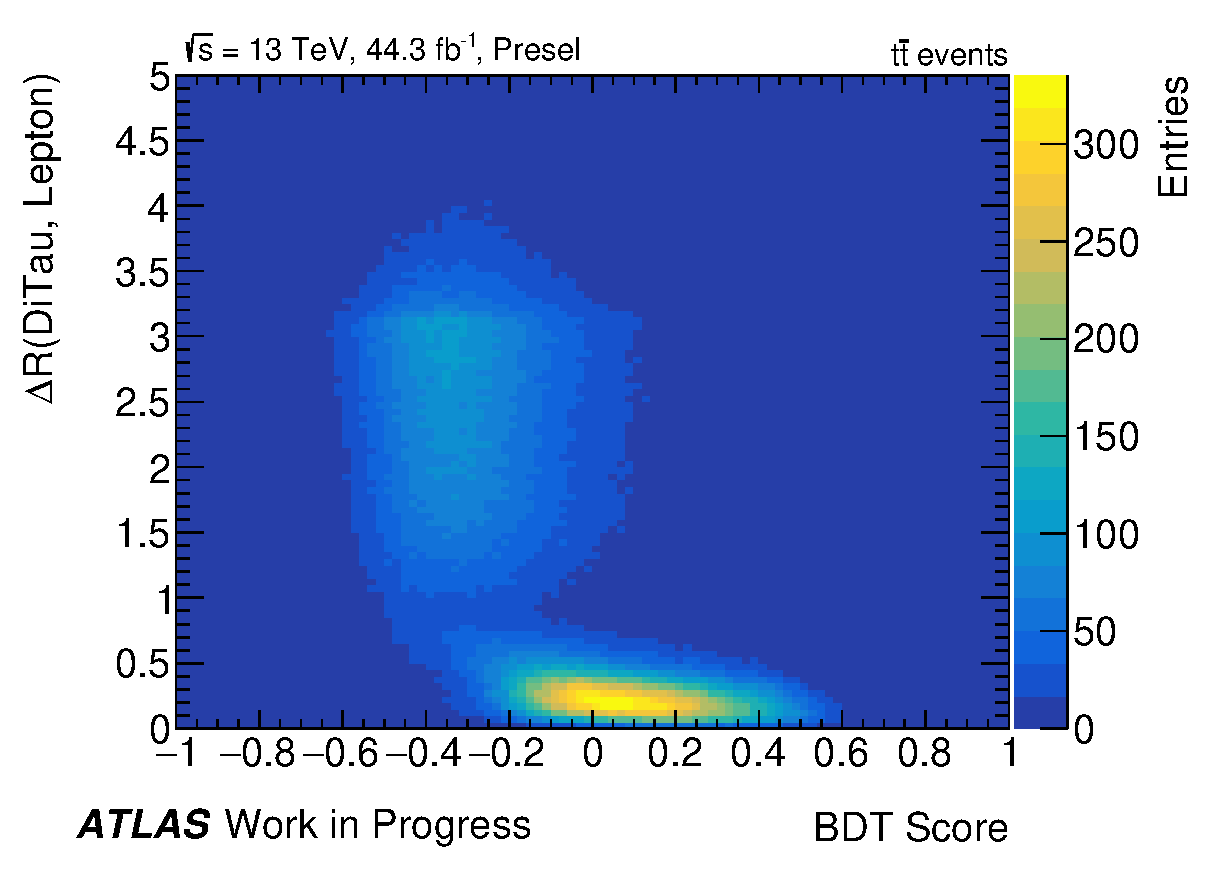
\includegraphics[width=0.99\linewidth]{Assets/Plots/Presel/h_mc16d_ttbar_ditau_bdt_lepton_dr.eps}\\

    \noindent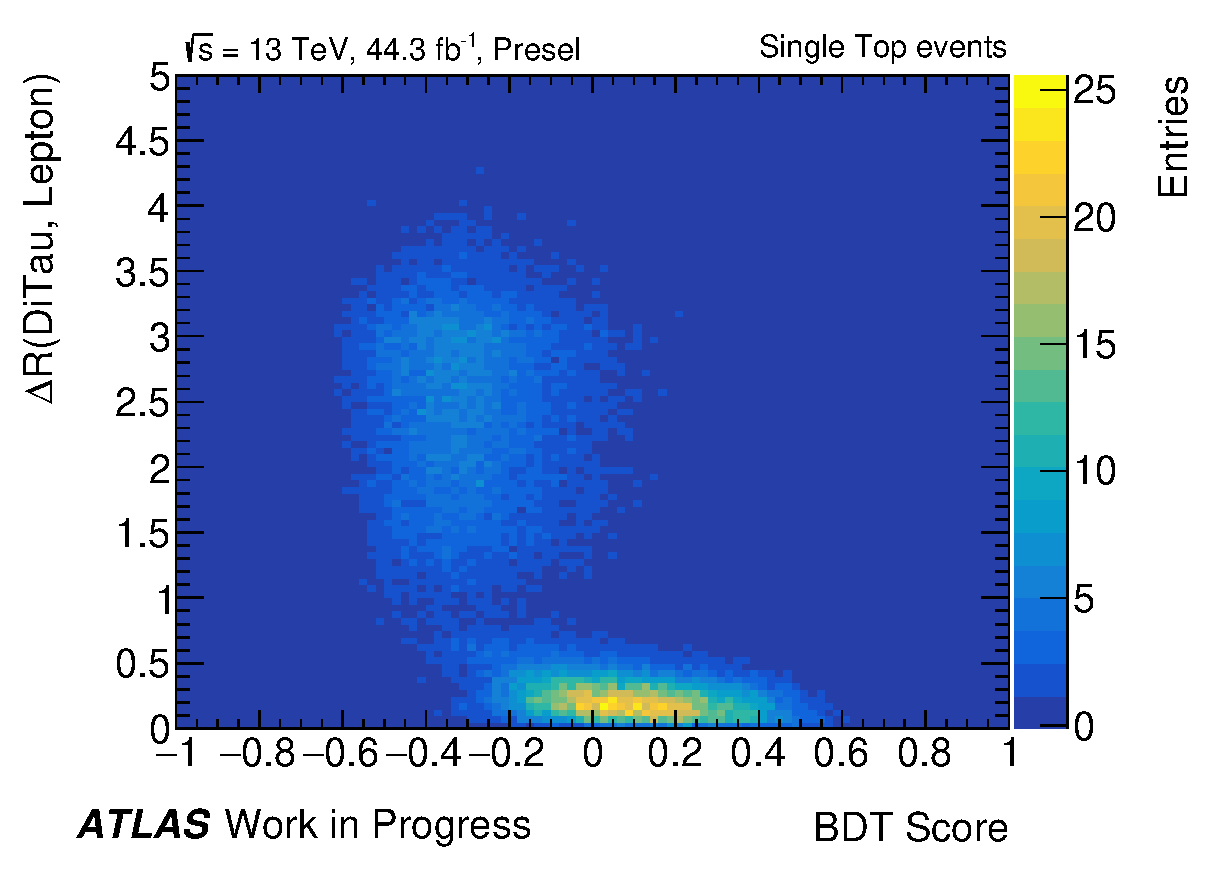
\includegraphics[width=0.99\linewidth]{Assets/Plots/Presel/h_mc16d_SingleTop_ditau_bdt_lepton_dr.eps}\\

    \noindent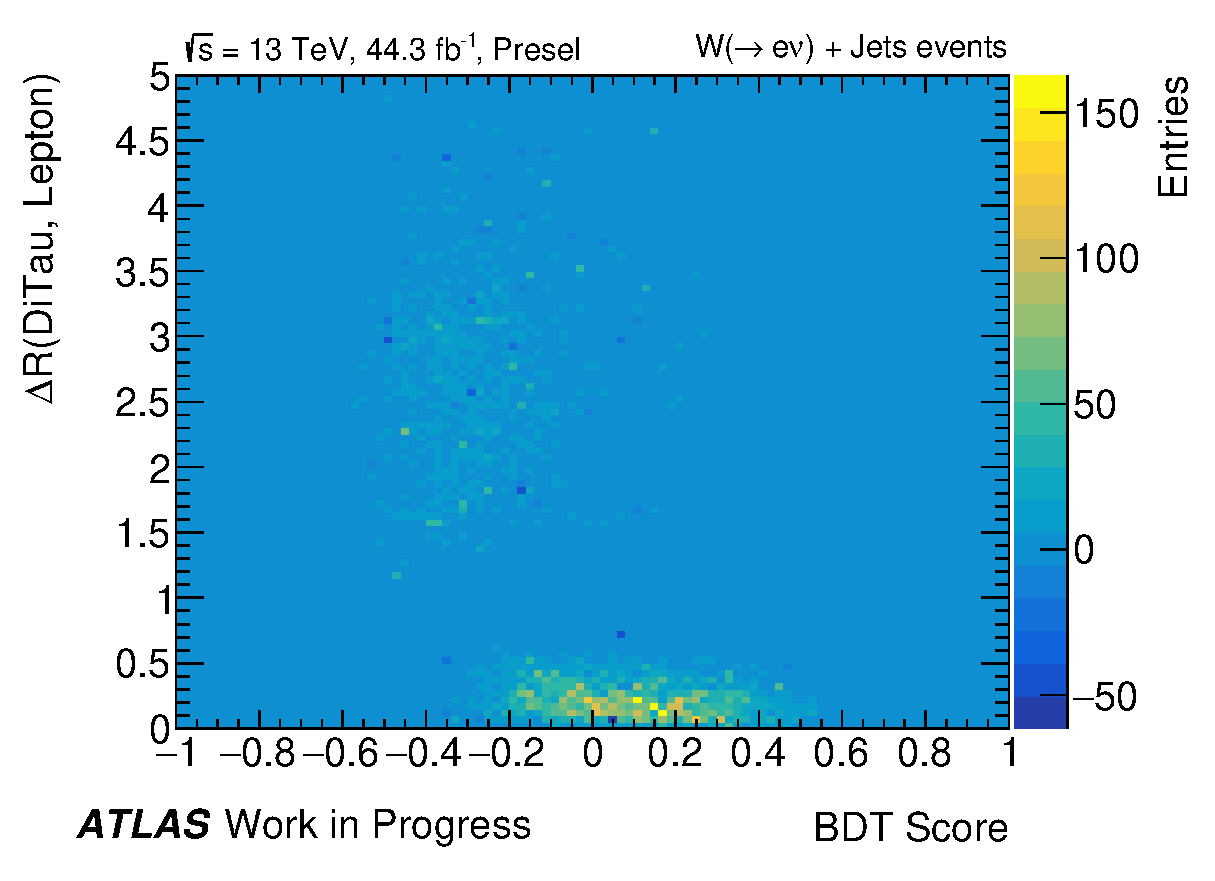
\includegraphics[width=0.99\linewidth]{Assets/Plots/Presel/h_mc16d_WjetsEnu_ditau_bdt_lepton_dr.eps}
    \caption{Distribuciones de $BDT$ vs $\Delta R(\text{DiTau}, \text{Lepton})$, para muestras MC de $t\bar{t}$, SingleTop y $W(\to ee) + Jets$, utilizando solo cortes de preselección.}
    \label{fig:ch4:presel:h_ditau_bdt_lepton_dr}
\end{marginfigure}

A diferencia de los DiTau \text{fake} originados en jets de QCD, donde la mayoría se encuentran en $BDT < 0$, la identificación de los objetos DiTau no tiene un buen poder discriminante contra leptones. Los cúmulos conformados por estos objetos, en la región $\Delta R < 1.0$ y $-0.4 < BDT < 0.6$, se solapan con el intervalo $BDT > 0.22$, en el que definimos preliminarmente la SR. Por lo tanto, se propone realizar un OR adicional entre leptones y DiTaus, priorizando los primeros, por medio de un corte $\Delta R > 1.0$ para su total eliminación en todas las regiones.






\noFBSection{Definición preliminar de la Región de Señal}

Como se ha adelantado, en este análisis la principal variable de selección para discriminar eventos de señal y fondo es el resultado del BDT de indentificación de los objetos DiTau. Siguiendo el criterio de 1\% de aceptancia de eventos del fondo dominante $t\bar{t}$, correspondiéndose a una eficiencia media de la señal de 75\%, introducimos el corte preliminar $BDT > 0.22$ para todos los objetos que pertenezcan a la SR.

\begin{marginfigure}
    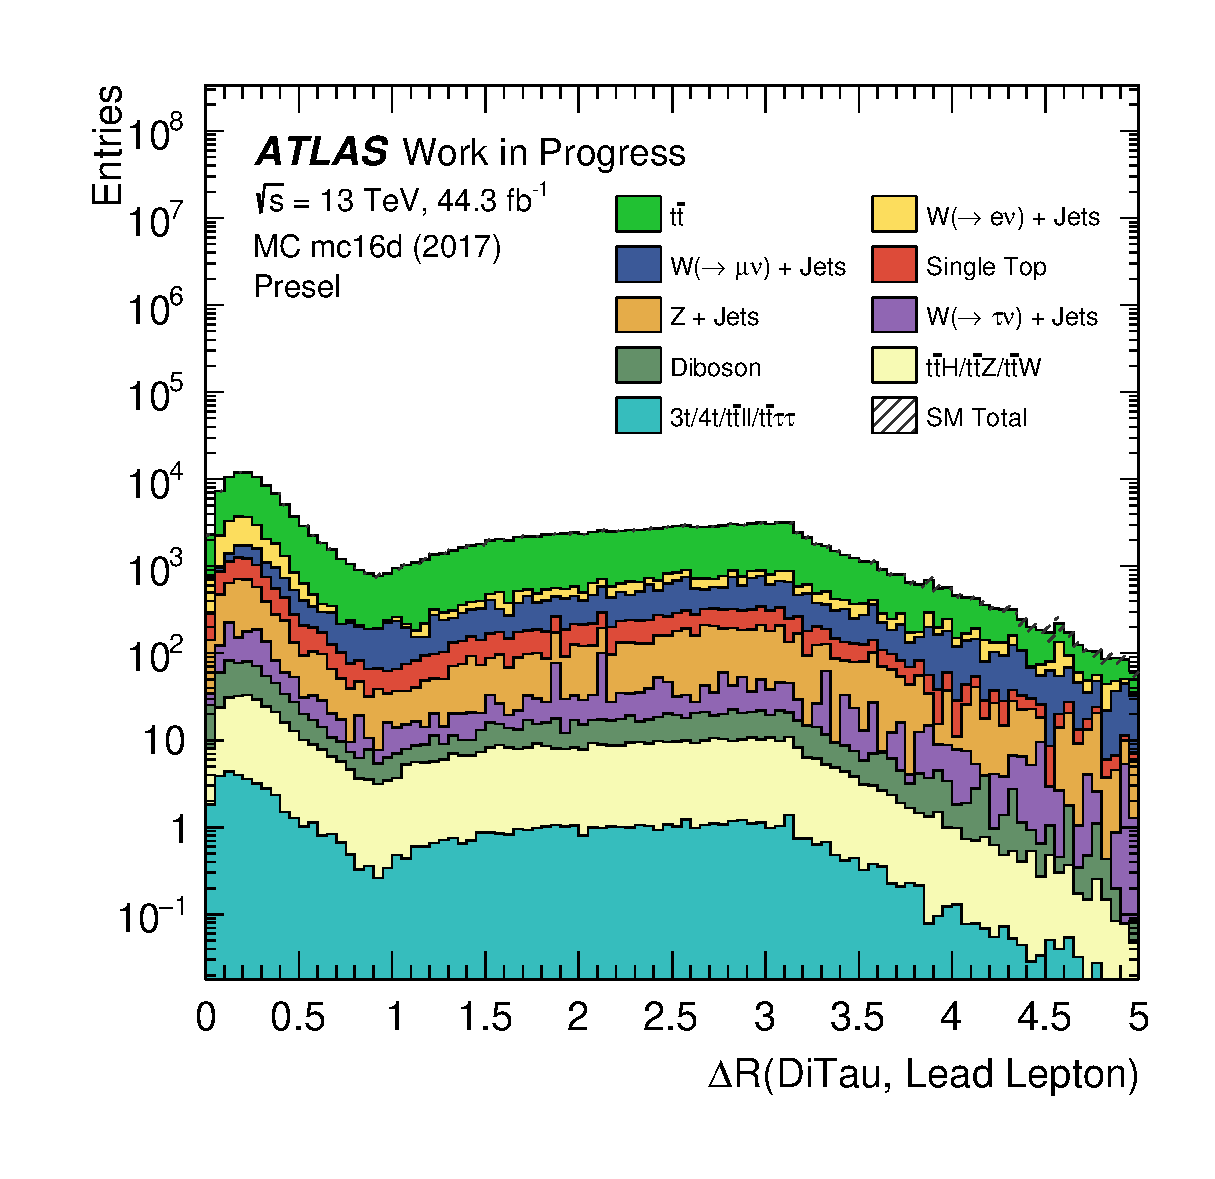
\includegraphics[width=0.99\linewidth]{Assets/Plots/Presel/h_stack_mc16d_ditau_lepton_dr.eps}
    \caption{Distribución de $\Delta R(\text{DT}, \text{Lepton})$, con solo cortes de preselección.}
    \label{fig:ch4:presel:h_ditau_lepton_dr}
\end{marginfigure}

En esta región se espera que los candidatos DiTau sean producidos por un par $\tau^+_{\text{had}} \tau^-_{\text{had}}$. Por lo tanto, se puede añadir una selección adicional en la carga de los subjets LyS del DiTau, requiriendo que además de ser $\abs{q} == 1$, sus signos sean opuestos. Esto suprime aproximadamente el 50\% de los eventos de fondo, donde no se supone una preferencia por un signo particular de la carga.

Los 4 jets producidos en el decaimiento semileptónico del par $t\bar{t}$ (2 de los cuales deberán ser etiquetados como b-jets) nos permiten reducir aún más la contaminación de fondos disímiles al estado final de los eventos $t\bar{t}(X\to\tau\tau)$, exhibido en la \cref{fig:ch4:ttX_diagram}. Si bien podríamos incrementar el corte en el número de jets hasta $NJets \geq 4$ y $NBJets \geq 2$, se optó por reducir preliminarmente este requerimiento a $NJets \geq 3$ y $NBJets \geq 1$, para evitar el rechazo de eventos donde 1 jet o b-jet ha sido mal identificado.

La baja sección eficaz de la señal, junto a la topología de los eventos $t\bar{t}X$, sugiere que solo deberíamos encontrar 1 objeto DiTau correctamente identificados por evento. Más aún, el OR aplicado contra los leptones y la selección más estricta en el número de jets y b-jets por evento, restringen fuertemente la posibilidad de reconstruir un objeto DiTau \textit{fake} adicional. Introduciremos entonces un corte final $NDiTau == 1$.

La presencia de neutrinos en el estado final, provenientes del decaimiento semileptónico del $t\bar{t}$ asociado a la producción del $X$ y del decaimiento de los \thads, sugieren la presencia de grandes candidades de $E_T^{\text{miss}}$ en los eventos de señal. Además, debido al \textit{boosteo} del $X$, los neutrinos producidos por el par de \thads se encontrarían principalmente orientados en la dirección del objeto DiTau. Esta última correlación puede ser detectada en la variable angular $\Delta\phi(E_T^{\text{miss}}, \text{DiTau})$. La elección de los cortes en estas dos variables está siendo actualmente estudiada, mediante una optimización numérica de todos los cortes de definición de la SR maximizando la significancia esperada de descubrimiento.

\begin{margintable}[-5em]
    \begin{tabular}{L{40mm} l}
\toprule
                                                 & \multicolumn{1}{c}{SR} \\
\midrule
Preselección                                     & $\checkmark$           \\
$NJets$                                          & $\geq 3$               \\
$NBJets$                                         & $\geq 1$               \\
$\Delta R(\text{DiTau}, \text{Baseline Lepton})$ & $\geq 1.0$             \\
$q_{\text{lead}} q_{\text{sublead}}$             & $-1$                   \\
DiTau $BDT$                                      & $\geq 0.22$            \\
$NDiTau$                                         & 1                      \\
\bottomrule
\end{tabular}
    \caption{Definición preliminar de la SR. Los cortes se aplican en el orden enlistado en la tabla. Los cortes en $NJetsTot$ y $NBJets$ se realizan luego del OR entre (B)Jets y DiTaus ($\Delta R(\text{DiTau}, \text{(B)Jet}) > 1$).}
    \label{tbl:ch4:SR:definition}
\end{margintable}

Un resumen de la definición completa de la SR preliminar se encuentra en la \cref{tbl:ch4:SR:definition}.

\noFBSubsection{Distribuciones de eventos} \label{sec:ch4:SR:results}

Como observamos en la \cref{tbl:ch4:SR:yields}, el fondo $t\bar{t}$ permanece dominante en la SR, alcanzando más del 77\% del total, aunque con una significativa reducción del número de eventos sobre los cortes de preselección. Las siguientes contribuciones, en orden descendiente de importancia, son $W(\to\ell\nu) + Jets$, $Z(\to\ell\ell) + Jets$ y SingleTop. Las discrepancias entre los canales de decaimiento leptónicos ($e$ y $\mu$) de los bosones $W$ y $Z$ puede ser atribuida a diferencias en las eficiencias de los triggers y procesos de reconstrucción de los electrones y muones.

\begin{margintable}[5em]
    \setlength{\tabcolsep}{0.8mm}
    \begin{tabular}{L{26mm} rr}
\toprule
                         & \multicolumn{2}{c}{SR}                 \\
\midrule
$t\bar{t}$               & 583.833              & ( 77.204\%)     \\
$W(\to \mu\nu) + Jets$   & 39.071               & (  5.167\%)     \\
$Single Top$             & 26.162               & (  3.460\%)     \\
$W(\to e\nu) + Jets$     & 20.259               & (  2.679\%)     \\
$W(\to \tau\nu) + Jets$  & 3.708                & (  0.490\%)     \\
$Z(\to \mu\mu) + Jets$   & 41.298               & (  5.461\%)     \\
$t\bar{t}H$              & 2.226                & (  0.294\%)     \\
$t\bar{t}Z$              & 0.994                & (  0.131\%)     \\
$Z(\to ee) + Jets$       & 23.116               & (  3.057\%)     \\
$t\bar{t}W$              & 1.532                & (  0.203\%)     \\
$Diboson$                & 2.701                & (  0.357\%)     \\
$Z(\to \tau\tau) + Jets$ & 7.340                & (  0.971\%)     \\
$4t$                     & 0.110                & (  0.015\%)     \\
$t\bar{t}\mu\mu$         & 0.776                & (  0.103\%)     \\
$t\bar{t}\tau\tau$       & 2.594                & (  0.343\%)     \\
$t\bar{t}ee$             & 0.485                & (  0.064\%)     \\
$3t$                     & 0.019                & (  0.003\%)     \\
\textbf{Total}           & \textbf{756.226}     &                 \\
\midrule
\SI{20}{\GeV} $X$        & 0.102                &                 \\
\SI{40}{\GeV} $X$        & 0.255                &                 \\
\SI{60}{\GeV} $X$        & 0.273                &                 \\
\bottomrule
\end{tabular}
    \vspace{1em}
    \caption{Composición de los fondos contaminantes y señal en la SR preliminar. Se utilizaron solo muestras de \texttt{mc16d}, normalizadas a la luminosidad integrada del año 2017.}
    \label{tbl:ch4:SR:yields}
\end{margintable}

En la SR preliminar, la mayor reducción en el número de eventos en el fondo $t\bar{t}$ es encontrada en el corte en el $BDT$ de los DiTaus, donde solo un 2.1\% de los eventos satisface el corte (\cref{tbl:ch4:SR:cutflows}). En las distribuciones de $BDT$ en la SR (\cref{fig:ch4:SR:h_ditaus}, aplicando todos los cortes de la SR, excepto la selección en $BDT$) observamos una meseta de eventos de señal en el intervalo $BDT < 0$. Esta diferencia respecto a las distribuciones del entrenamiento del BDT (\cref{fig:ch3:ditau:bdt_output}) está formada por objetos DiTau \textit{fake}, producidos por Jets de QCD.

\begin{figure*}[t]
    \centering\noindent
    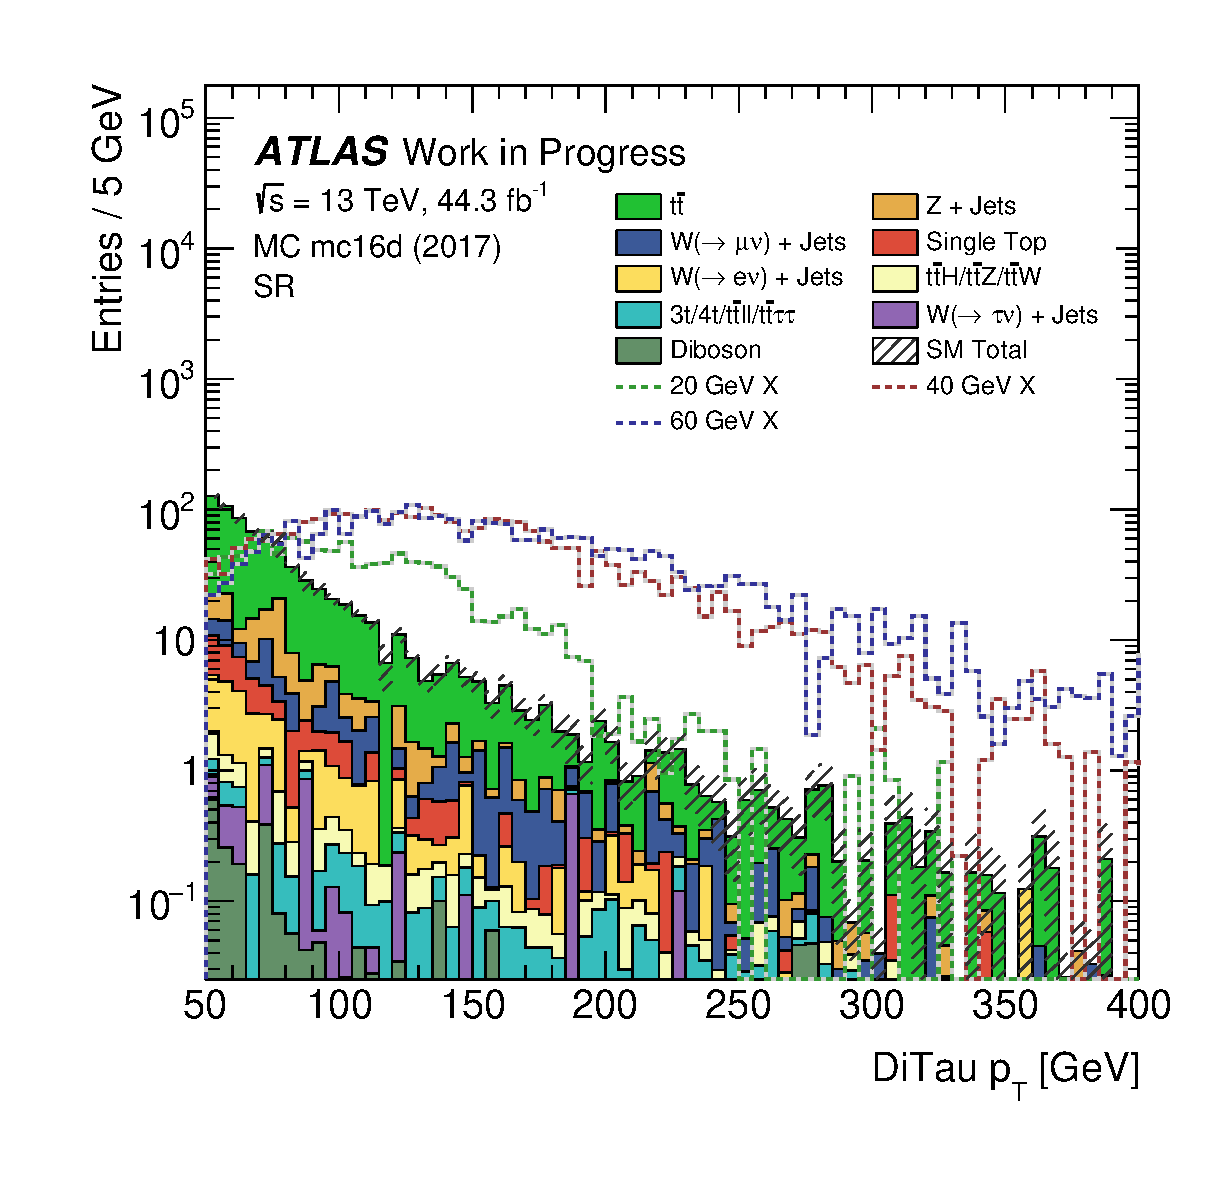
\includegraphics[width=0.49\fulllinewidth]{Assets/Plots/SR/h_stack_mc16d_ditau_pt.eps}
    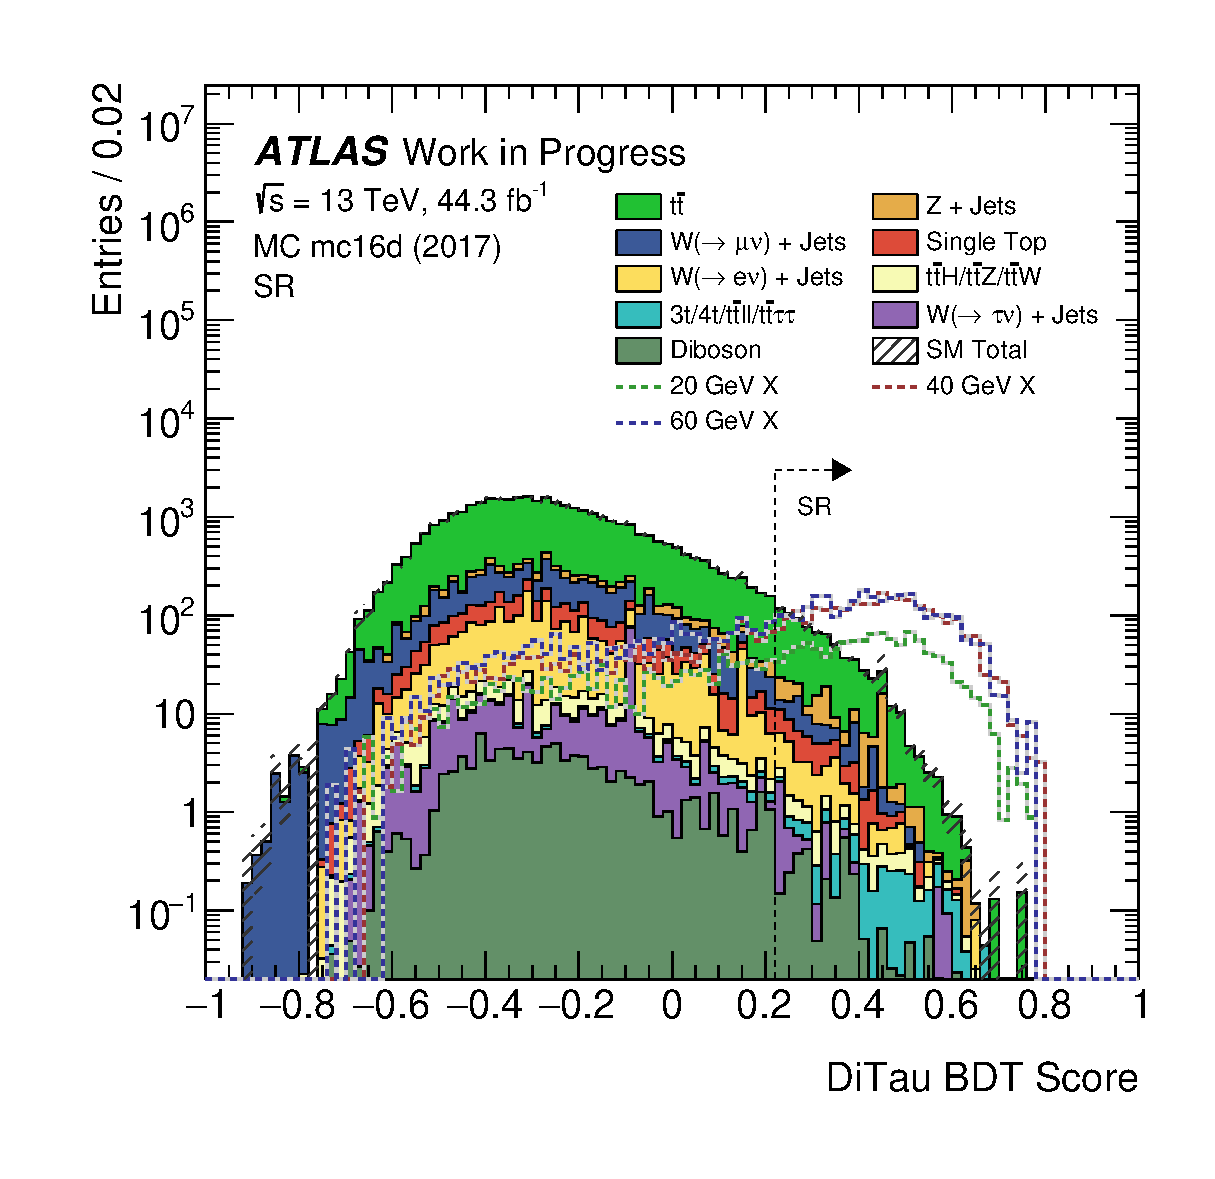
\includegraphics[width=0.49\fulllinewidth]{Assets/Plots/SR/h_stack_mc16d_ditau_bdt.eps}

    \caption{Distribuciones de $p_T$ y $BDT$ de los objetos DiTau en la SR. La flecha en la distribución de $BDT$ indica el corte de definición de la SR. Las muestras de señal han sido escaladas por $10^4$.}
    \label{fig:ch4:SR:h_ditaus}
\end{figure*}

En las muestras de señal, la mayor reducción de eventos en la SR se da por los cortes de calidad y cinemáticos de los objetos DiTau. Bajo esta definición de la región, eliminar el corte en el número de DiTaus no produce un cambio en el número final de eventos.

Para estudiar la composición de los objetos DiTau, se efectuó un \textit{truth match} (TM) entre los candidatos DiTau reconstruidos, e información de las partículas verdaderas (\textit{truth}) provistas por el generador. Se requirió que estas se encuentren dentro del objeto DiTau, es decir, a una distancia $\Delta R < 1.0$ de su baricentro.

En todos los procesos de fondo, la mayor parte de los objetos DiTau en la SR se encuentran conformados por jets provenientes de la produción de quarks y otros procesos de QCD (\cref{tbl:ch4:SR:ditau_composition} y \cref{fig:ch4:SR:ditau_composition}). El corte $\Delta R(\text{DiTau}, \text{Lepton}) > 1$ en la SR excluye los objetos DiTau \textit{fake} originados en electrones y muones. Sin embargo, todavía encontramos un $6\%$ de eventos donde el objeto DiTau se ha reconstruido a partir de un par de \ttaus decayendo leptónicamente. Esto puede ocurrir en casos donde el leptón producido en el decaimiento del \ttau no supera el corte de energía mínima de $p_T > \SI{27}{\GeV}$, no siendo incluido en los objetos utilizados en el análisis del evento, o ante una mala reconstrucción e identificación de los leptones en el estado final de la interacción. Menos del 1\% de los eventos se corresponden a pares de \ttaus decayendo hadrónicamente, como los objetos de señal esperados.

En las muestras de señal, la mayoría de los eventos contienen un objeto DiTau vinculado con el par de \thads obtenido en el decaimiento del pseudoescalar $X$. Los objetos DiTau con un único \thad en su interior son, en gran proporción, también originados en el $X$, aunque con la producción de un único \thad y un tau en decaimiento leptónico.

\begin{marginfigure}[8em]
    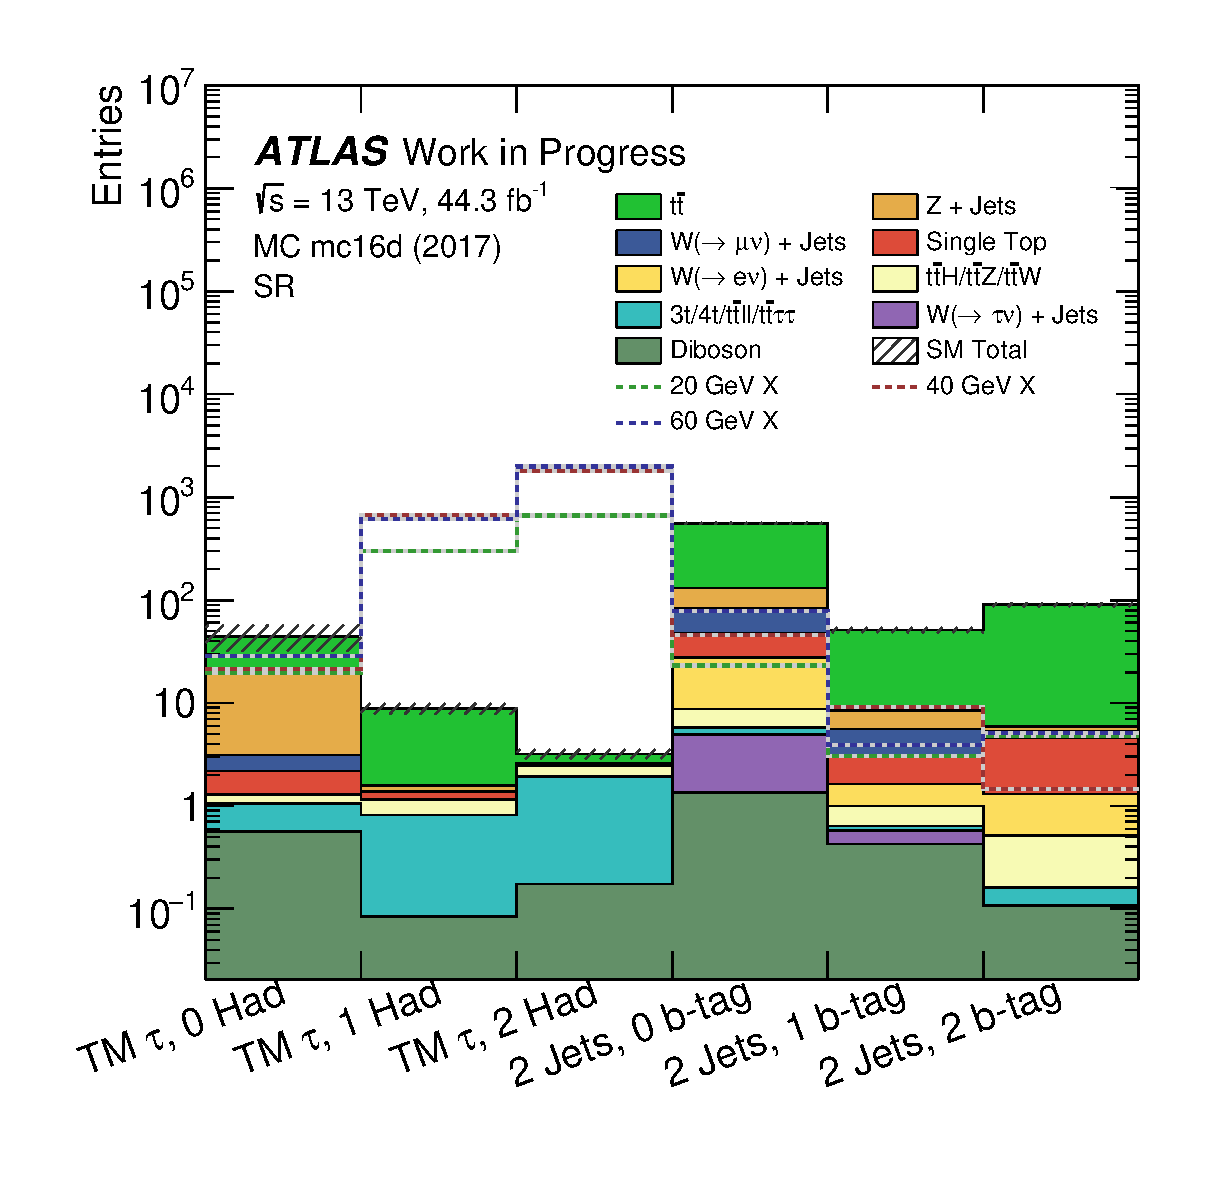
\includegraphics[width=0.99\linewidth]{Assets/Plots/SR/h_stack_mc16d_ditau_composition.eps}
    \caption{Composición de los objetos DiTau en la SR. Las muestras de señal han sido escaladas por $10^4$. El \textit{truth match} se realizó respecto al jet externo $R = 1$ del objeto DiTau.}
    \label{fig:ch4:SR:ditau_composition}
\end{marginfigure}

\clearpage{}
\begin{table*}[th!]
    \subfloat[][\label{tbl:ch4:SR:cutflows:ttbar}]{
    \centering
    \begin{minipage}{0.49\linewidth}
        \centering
        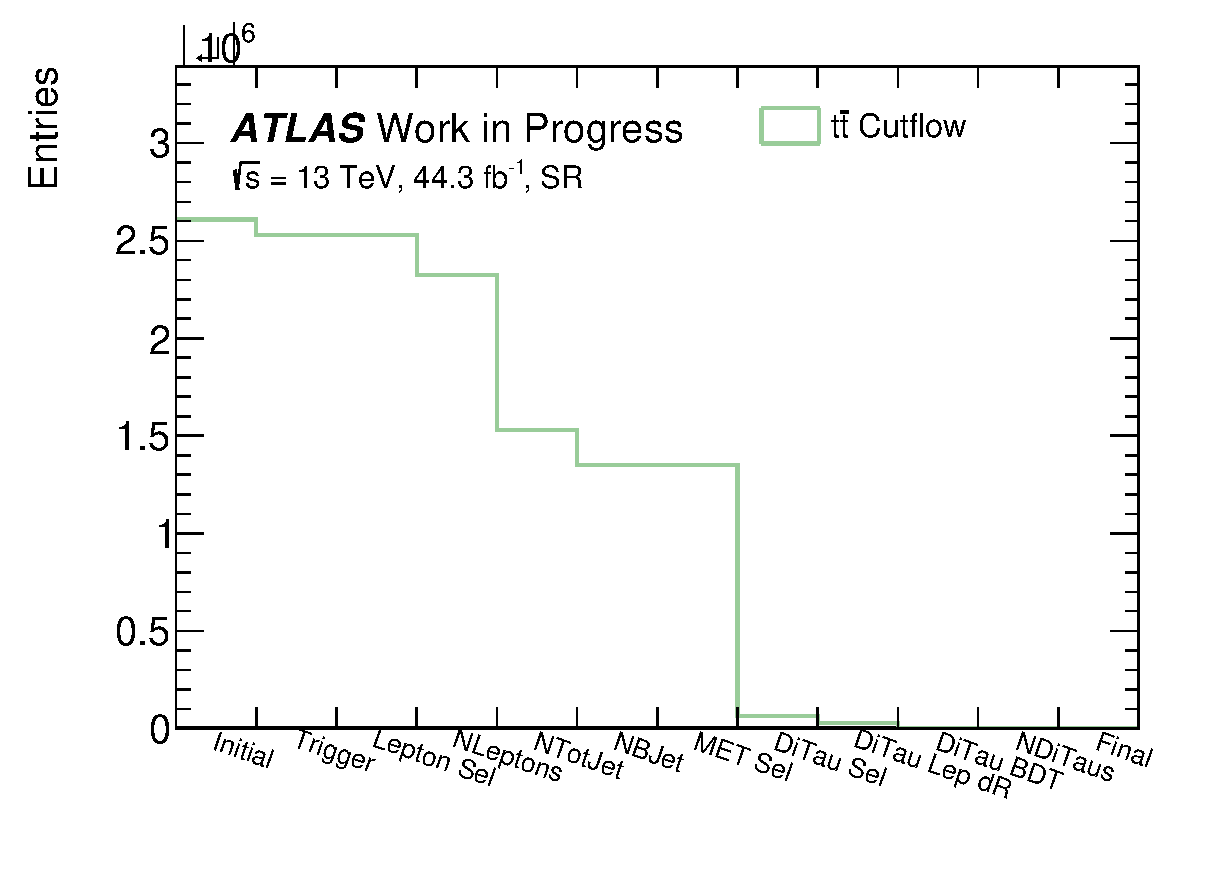
\includegraphics[width=0.8\linewidth]{Assets/Plots/SR/h_mc16d_ttbar_cutflow_weighted.eps}
    \end{minipage}
    \begin{minipage}{0.49\linewidth}
        \centering
        \small
        \setlength{\tabcolsep}{10pt}
        \vspace{-2em}
        \begin{tabular}{lrr}
\toprule
Initial        & 2609591.154       & (100.00\%)         \\
Trigger        & 2528568.531       & (96.90\%)          \\
Lepton Sel     & 2528171.500       & (96.88\%)          \\
NLeptons       & 2321677.922       & (88.97\%)          \\
NTotJet        & 1531255.463       & (58.68\%)          \\
NBJet          & 1350146.213       & (51.74\%)          \\
MET Sel        & 1350146.213       & (51.74\%)          \\
DiTau Sel      & 62825.557         & (2.41\%)           \\
DiTau Lep dR   & 28060.804         & (1.08\%)           \\
DiTau BDT      & 583.833           & (0.02\%)           \\
NDiTaus        & 583.833           & (0.02\%)           \\
\textbf{Final} & \textbf{583.833}  & \textbf{(0.02\%)}  \\
\bottomrule
\end{tabular}
    \end{minipage}
    }

    \subfloat[][\label{tbl:ch4:SR:cutflows:signal}]{
        \begin{minipage}{0.98\linewidth}
            \centering
            \small
            \setlength{\tabcolsep}{3mm}
            \begin{tabular}{lrrrrrrrrr}
\toprule
               & & \multicolumn{2}{c}{\SI{20}{\GeV} $X$} & & \multicolumn{2}{c}{\SI{40}{\GeV} $X$} & & \multicolumn{2}{c}{\SI{60}{\GeV} $X$} \\
\midrule
Initial        & & 4.265          & (100.000\%)          & & 7.590          & (100.000\%)          & & 9.863          & (100.000\%)          \\
Trigger        & & 4.048          & ( 94.910\%)          & & 7.180          & ( 94.600\%)          & & 9.305          & ( 94.340\%)          \\
Lepton Sel     & & 4.047          & ( 94.890\%)          & & 7.178          & ( 94.570\%)          & & 9.303          & ( 94.320\%)          \\
NLeptons       & & 3.021          & ( 70.830\%)          & & 5.075          & ( 66.870\%)          & & 6.333          & ( 64.210\%)          \\
NTotJet        & & 2.102          & ( 49.280\%)          & & 3.462          & ( 45.610\%)          & & 4.363          & ( 44.240\%)          \\
NBJet          & & 1.819          & ( 42.650\%)          & & 2.956          & ( 38.950\%)          & & 3.745          & ( 37.980\%)          \\
MET Sel        & & 1.819          & ( 42.650\%)          & & 2.956          & ( 38.950\%)          & & 3.745          & ( 37.980\%)          \\
DiTau Sel      & & 0.260          & (  6.090\%)          & & 0.543          & (  7.150\%)          & & 0.655          & (  6.640\%)          \\
DiTau-Lep dR   & & 0.183          & (  4.290\%)          & & 0.398          & (  5.240\%)          & & 0.455          & (  4.610\%)          \\
DiTau-MET dPhi & & 0.183          & (  4.290\%)          & & 0.398          & (  5.240\%)          & & 0.455          & (  4.610\%)          \\
DiTau BDT      & & 0.102          & (  2.390\%)          & & 0.255          & (  3.360\%)          & & 0.273          & (  2.770\%)          \\
NDiTaus        & & 0.102          & (  2.390\%)          & & 0.255          & (  3.360\%)          & & 0.273          & (  2.770\%)          \\
Final          & & 0.102          & (  2.390\%)          & & 0.255          & (  3.360\%)          & & 0.273          & (  2.770\%)          \\
\bottomrule
\end{tabular}
            \vspace{1em}
        \end{minipage}
    }

    \fullwidthCaption{Cutflows de las muestras \texttt{mc16d} del fondo dominante $t\bar{t}$ \subref{tbl:ch4:SR:cutflows:ttbar} y las muestras de señal $t\bar{t}X$ \subref{tbl:ch4:SR:cutflows:signal} en la SR, normalizado a la luminosidad integrada del 2017. Todos los eventos fueron pesados con la eq. \eqref{eq:ch4:weight}. Trabajo en progreso.}
    \label{tbl:ch4:SR:cutflows}
\end{table*}

\begin{table*}[th!]
    \centering
    \footnotesize
    \setlength{\tabcolsep}{1.2mm}
    \begin{tabular}{lrrrrrrrrrr}
\toprule
                        & \multicolumn{2}{c}{$t\bar{t}$} & \multicolumn{2}{c}{Total SM} & \multicolumn{2}{c}{\SI{20}{\GeV} $X$} & \multicolumn{2}{c}{\SI{40}{\GeV} $X$} & \multicolumn{2}{c}{\SI{60}{\GeV} $X$} \\
\midrule
TM DiTaus, 0 subj. had. & 23.149        & (3.96\%)       & 44.648       & (5.90\%)      & 0.002             & (1.92\%)          & 0.002             & (0.85\%)          & 0.003             & (1.05\%)          \\
TM DiTaus, 1 subj. had. & 7.240         & (1.24\%)       & 8.824        & (1.17\%)      & 0.030             & (29.40\%)         & 0.066             & (25.96\%)         & 0.062             & (22.66\%)         \\
TM DiTaus, 2 subj. had. & 0.580         & (0.10\%)       & 3.209        & (0.42\%)      & 0.067             & (65.64\%)         & 0.181             & (70.98\%)         & 0.199             & (73.06\%)         \\
2 jets, 0 b-tagged      & 412.304       & (70.62\%)      & 557.902      & (73.78\%)     & 0.002             & (2.27\%)          & 0.005             & (1.79\%)          & 0.008             & (2.90\%)          \\
2 jets, 1 b-tagged      & 47.769        & (8.18\%)       & 51.280       & (6.78\%)      & $< 0.001$         & (0.30\%)          & $< 0.001$         & (0.36\%)          & $< 0.001$         & (0.14\%)          \\
2 jets, 2 b-tagged      & 92.781        & (15.89\%)      & 90.352       & (11.95\%)     & $< 0.001$         & (0.47\%)          & $< 0.001$         & (0.06\%)          & $< 0.001$         & (0.19\%)          \\
Total                   & 583.833       &                & 756.226      &               & 0.102             &                   & 0.255             &                   & 0.273             &                   \\
\bottomrule
\end{tabular}
    \vspace{1em}

    \fullwidthCaption{Composición de los objetos DiTau en la SR para los procesos de fondo ($t\bar{t}$ y el total de los fondos del SM) y señal. El \textit{truth match} se realizó respecto a los subjets \textit{leading} y \textit{subleading}, verificando que intersecten en $\Delta R < 0.2$ de su baricentro con los objetos del generador. Trabajo en progreso.}
    \label{tbl:ch4:SR:ditau_composition}
\end{table*}

\cleardoublepage{}